\documentclass[man,mask,floatsintext]{apa6}
\usepackage{lmodern}
\usepackage{amssymb,amsmath}
\usepackage{ifxetex,ifluatex}
\usepackage{fixltx2e} % provides \textsubscript
\ifnum 0\ifxetex 1\fi\ifluatex 1\fi=0 % if pdftex
  \usepackage[T1]{fontenc}
  \usepackage[utf8]{inputenc}
\else % if luatex or xelatex
  \ifxetex
    \usepackage{mathspec}
  \else
    \usepackage{fontspec}
  \fi
  \defaultfontfeatures{Ligatures=TeX,Scale=MatchLowercase}
\fi
% use upquote if available, for straight quotes in verbatim environments
\IfFileExists{upquote.sty}{\usepackage{upquote}}{}
% use microtype if available
\IfFileExists{microtype.sty}{%
\usepackage{microtype}
\UseMicrotypeSet[protrusion]{basicmath} % disable protrusion for tt fonts
}{}
\usepackage{hyperref}
\hypersetup{unicode=true,
            pdftitle={Supplementary materials: Modeling the influence of language input statistics on children's speech production},
            pdfauthor={Ingeborg Roete, Stefan L. Frank, Paula Fikkert, \& Marisa Casillas},
            pdfkeywords={statistical learning, language learning, abstraction, developmental
trajectory, age-invariance, CHILDES, children},
            pdfborder={0 0 0},
            breaklinks=true}
\urlstyle{same}  % don't use monospace font for urls
\usepackage{graphicx}
% grffile has become a legacy package: https://ctan.org/pkg/grffile
\IfFileExists{grffile.sty}{%
\usepackage{grffile}
}{}
\makeatletter
\def\maxwidth{\ifdim\Gin@nat@width>\linewidth\linewidth\else\Gin@nat@width\fi}
\def\maxheight{\ifdim\Gin@nat@height>\textheight\textheight\else\Gin@nat@height\fi}
\makeatother
% Scale images if necessary, so that they will not overflow the page
% margins by default, and it is still possible to overwrite the defaults
% using explicit options in \includegraphics[width, height, ...]{}
\setkeys{Gin}{width=\maxwidth,height=\maxheight,keepaspectratio}
\IfFileExists{parskip.sty}{%
\usepackage{parskip}
}{% else
\setlength{\parindent}{0pt}
\setlength{\parskip}{6pt plus 2pt minus 1pt}
}
\setlength{\emergencystretch}{3em}  % prevent overfull lines
\providecommand{\tightlist}{%
  \setlength{\itemsep}{0pt}\setlength{\parskip}{0pt}}
\setcounter{secnumdepth}{0}
% Redefines (sub)paragraphs to behave more like sections
\ifx\paragraph\undefined\else
\let\oldparagraph\paragraph
\renewcommand{\paragraph}[1]{\oldparagraph{#1}\mbox{}}
\fi
\ifx\subparagraph\undefined\else
\let\oldsubparagraph\subparagraph
\renewcommand{\subparagraph}[1]{\oldsubparagraph{#1}\mbox{}}
\fi

%%% Use protect on footnotes to avoid problems with footnotes in titles
\let\rmarkdownfootnote\footnote%
\def\footnote{\protect\rmarkdownfootnote}


  \title{Supplementary materials: Modeling the influence of language input
statistics on children's speech production}
    \author{Ingeborg Roete\textsuperscript{1,2}, Stefan L. Frank\textsuperscript{2},
Paula Fikkert\textsuperscript{2}, \& Marisa Casillas\textsuperscript{1}}
    \date{}
  
\shorttitle{SM: Modeling input statistics in child speech productions}
\affiliation{
\vspace{0.5cm}
\textsuperscript{1} Max Planck Institute for Psycholinguistics\\\textsuperscript{2} Radboud University}
\keywords{statistical learning, language learning, abstraction, developmental trajectory, age-invariance, CHILDES, children}
\usepackage{csquotes}
\usepackage{upgreek}
\captionsetup{font=singlespacing,justification=justified}

\usepackage{longtable}
\usepackage{lscape}
\usepackage{multirow}
\usepackage{tabularx}
\usepackage[flushleft]{threeparttable}
\usepackage{threeparttablex}

\newenvironment{lltable}{\begin{landscape}\begin{center}\begin{ThreePartTable}}{\end{ThreePartTable}\end{center}\end{landscape}}

\makeatletter
\newcommand\LastLTentrywidth{1em}
\newlength\longtablewidth
\setlength{\longtablewidth}{1in}
\newcommand{\getlongtablewidth}{\begingroup \ifcsname LT@\roman{LT@tables}\endcsname \global\longtablewidth=0pt \renewcommand{\LT@entry}[2]{\global\advance\longtablewidth by ##2\relax\gdef\LastLTentrywidth{##2}}\@nameuse{LT@\roman{LT@tables}} \fi \endgroup}


\usepackage{lineno}

\linenumbers

\authornote{

Correspondence concerning this article should be addressed to Marisa
Casillas, Wundtlaan 1, 6525 XD, Nijmegen, The Netherlands. E-mail:
\href{mailto:marisa.casillas@mpi.nl}{\nolinkurl{marisa.casillas@mpi.nl}}}

\abstract{

}

\begin{document}
\maketitle

\section{Full model output of main text
analyses}\label{full-model-output-of-main-text-analyses}

\textbf{Below readers will find the full statistical model output for
each of the six models reported in the main text (that is, one for local
input and one for cumulative input for each of the three analyses:
uncorrected likelihood of accurate reconstruction, corrected
reconstruction accuracy, and likelihood of unseen words).}

\pagebreak

\begin{table}[tbp]
\begin{center}
\begin{threeparttable}
\caption{\label{tab:tab-uncorr_reconstr_acc-local-MAIN}**Full model output for the analysis of uncorrected reconstruction accuracy using local speech input.**}
\begin{tabular}{lllllll}
\toprule
effect & \multicolumn{1}{c}{group} & \multicolumn{1}{c}{term} & \multicolumn{1}{c}{estimate} & \multicolumn{1}{c}{std.error} & \multicolumn{1}{c}{statistic} & \multicolumn{1}{c}{p.value}\\
\midrule
fixed & NA & (Intercept) & 2.59 & 0.50 & 5.19 & 0.00\\
fixed & NA & age & -0.81 & 0.18 & -4.44 & 0.00\\
ran\_pars & child & sd\_\_(Intercept) & 1.36 & NA & NA & NA\\
ran\_pars & child & sd\_\_age & 0.49 & NA & NA & NA\\
ran\_pars & child & cor\_\_(Intercept).age & -0.97 & NA & NA & NA\\
\bottomrule
\end{tabular}
\end{threeparttable}
\end{center}
\end{table}

\begin{table}[tbp]
\begin{center}
\begin{threeparttable}
\caption{\label{tab:tab-uncorr_reconstr_acc-cumu-MAIN}**Full model output for the analysis of uncorrected reconstruction accuracy using cumulative speech input.**}
\begin{tabular}{lllllll}
\toprule
effect & \multicolumn{1}{c}{group} & \multicolumn{1}{c}{term} & \multicolumn{1}{c}{estimate} & \multicolumn{1}{c}{std.error} & \multicolumn{1}{c}{statistic} & \multicolumn{1}{c}{p.value}\\
\midrule
fixed & NA & (Intercept) & 2.40 & 0.39 & 6.09 & 0.00\\
fixed & NA & age & -0.82 & 0.14 & -5.83 & 0.00\\
ran\_pars & child & sd\_\_(Intercept) & 1.18 & NA & NA & NA\\
ran\_pars & child & sd\_\_age & 0.41 & NA & NA & NA\\
ran\_pars & child & cor\_\_(Intercept).age & -0.96 & NA & NA & NA\\
\bottomrule
\end{tabular}
\end{threeparttable}
\end{center}
\end{table}

\begin{table}[tbp]
\begin{center}
\begin{threeparttable}
\caption{\label{tab:tab-corr_reconstr_acc-local-MAIN}**Full model output for the analysis of corrected reconstruction accuracy using local speech input.**}
\begin{tabular}{lllllll}
\toprule
effect & \multicolumn{1}{c}{group} & \multicolumn{1}{c}{term} & \multicolumn{1}{c}{estimate} & \multicolumn{1}{c}{std.error} & \multicolumn{1}{c}{statistic} & \multicolumn{1}{c}{p.value}\\
\midrule
fixed & NA & (Intercept) & 0.11 & 0.02 & 5.06 & NA\\
fixed & NA & recentered\_age & 0.03 & 0.02 & 1.68 & NA\\
ran\_pars & child & sd\_\_(Intercept) & 0.05 & NA & NA & NA\\
ran\_pars & child & sd\_\_recentered\_age & 0.04 & NA & NA & NA\\
ran\_pars & child & cor\_\_(Intercept).recentered\_age & 0.63 & NA & NA & NA\\
ran\_pars & Residual & sd\_\_Observation & 0.63 & NA & NA & NA\\
\bottomrule
\end{tabular}
\end{threeparttable}
\end{center}
\end{table}

\begin{table}[tbp]
\begin{center}
\begin{threeparttable}
\caption{\label{tab:tab-corr_reconstr_acc-cumu-MAIN}**Full model output for the analysis of corrected reconstruction accuracy using cumulative speech input.**}
\begin{tabular}{lllllll}
\toprule
effect & \multicolumn{1}{c}{group} & \multicolumn{1}{c}{term} & \multicolumn{1}{c}{estimate} & \multicolumn{1}{c}{std.error} & \multicolumn{1}{c}{statistic} & \multicolumn{1}{c}{p.value}\\
\midrule
fixed & NA & (Intercept) & 0.06 & 0.01 & 6.24 & NA\\
fixed & NA & recentered\_age & 0.02 & 0.01 & 1.59 & NA\\
ran\_pars & child & sd\_\_(Intercept) & 0.02 & NA & NA & NA\\
ran\_pars & child & sd\_\_recentered\_age & 0.03 & NA & NA & NA\\
ran\_pars & child & cor\_\_(Intercept).recentered\_age & -0.71 & NA & NA & NA\\
ran\_pars & Residual & sd\_\_Observation & 0.59 & NA & NA & NA\\
\bottomrule
\end{tabular}
\end{threeparttable}
\end{center}
\end{table}

\begin{table}[tbp]
\begin{center}
\begin{threeparttable}
\caption{\label{tab:tab-unseen_words-local-MAIN}**Full model output for the analysis of likelihood that a word in the child's speech was seen during training.**}
\begin{tabular}{lllllll}
\toprule
effect & \multicolumn{1}{c}{group} & \multicolumn{1}{c}{term} & \multicolumn{1}{c}{estimate} & \multicolumn{1}{c}{std.error} & \multicolumn{1}{c}{statistic} & \multicolumn{1}{c}{p.value}\\
\midrule
fixed & NA & (Intercept) & 3.13 & 0.33 & 9.64 & 0.00\\
fixed & NA & age & -0.55 & 0.11 & -5.00 & 0.00\\
ran\_pars & child & sd\_\_(Intercept) & 0.74 & NA & NA & NA\\
ran\_pars & child & sd\_\_age & 0.25 & NA & NA & NA\\
ran\_pars & child & cor\_\_(Intercept).age & -0.94 & NA & NA & NA\\
\bottomrule
\end{tabular}
\end{threeparttable}
\end{center}
\end{table}

\begin{table}[tbp]
\begin{center}
\begin{threeparttable}
\caption{\label{tab:tab-unseen_words-cumu-MAIN}**Full model output for the analysis of number of utterances with previously unheard words using cumulative speech input.**}
\begin{tabular}{lllllll}
\toprule
effect & \multicolumn{1}{c}{group} & \multicolumn{1}{c}{term} & \multicolumn{1}{c}{estimate} & \multicolumn{1}{c}{std.error} & \multicolumn{1}{c}{statistic} & \multicolumn{1}{c}{p.value}\\
\midrule
fixed & NA & (Intercept) & 2.85 & 0.36 & 7.82 & 0.00\\
fixed & NA & age & -0.02 & 0.12 & -0.18 & 0.86\\
ran\_pars & child & sd\_\_(Intercept) & 0.78 & NA & NA & NA\\
ran\_pars & child & sd\_\_age & 0.25 & NA & NA & NA\\
ran\_pars & child & cor\_\_(Intercept).age & -0.96 & NA & NA & NA\\
\bottomrule
\end{tabular}
\end{threeparttable}
\end{center}
\end{table}

\pagebreak

\section{Results using the original McCauley and Christiansen (2011)
reconstruction
method}\label{results-using-the-original-mccauley-and-christiansen-2011-reconstruction-method}

\textbf{While our implementation of the CBL learner is identical to
McCauley and Christiansen's, o}ur implementation of the
\textbf{\emph{reconstruction task}} diverges slightly from
\textbf{theirs: we discard utterances with unknown words and instead
provide a second analysis focused on the number of these
\enquote{un-reconstructable} utterances across age. Our reasoning for
discarding utterances with unknown words was that there is no obvious
way to give them a valid default transition matrix with other existing
chunks. In contrast, McCauley and Christiansen (2011) built a new chunk
for each unknown word when reconstructing utterances. This chunk with
the unknown word was then assigned a BTP equal to zero with respect to
any other chunk in the utterance it originated from. In what follows,}
we present results using McCauley and Christiansen's (2011) original
reconstruction task method. \textbf{Because their reconstruction task
attempts to reconstruct all utterances, we do not also} provide analyses
of the number of utterances containing unknown words.

We analyzed the effect of child age on the model's reconstruction
abilities for the child utterances with a mixed-effects model, including
age as a fixed effect and a by-child random intercept with random slopes
of age.

First, we used the binary (1: reconstructed correctly, 0: not
reconstructed correctly) measure from McCauley \& Christiansen (2011,
2014). The model's average percentage of correctly reconstructed
utterances across children and age points was similar for the locally
and cumulatively sampled speech (local: mean = 61.3 \%, range across
children = 51.6\%--69.6\%; cumulative: mean = 59.4\%, range across
children = 50.8\%--68.4\%). The number of correctly reconstructed
utterances decreased with age, regardless of the sampling methods
(local: \(b = -0.939, SE = 0.174, p < 0.001\); cumulative:
\(b = -0.848, SE = 0.138, p < 0.001\); see
\protect\hyperlink{smfig1}{Figure 1}).

Second, we used our corrected, length-and-repetition-controlled
reconstruction score. The model's average reconstruction score across
children and age points was similar for the locally and cumulatively
sampled speech (local: mean = 0.12, SE = 0.01; cumulative: mean = 0.08,
SE = 0.01). As in the main text, we centered age in the model so that we
could investigate whether reconstruction was greater than chance level
at the average age in our sample (2;6 years). Using both sampling
methods, we found a significantly positive intercept (local sampling:
\(b = 0.130, SE = 0.016, t = 7.911\); cumulative sampling:
\(b = 0.0789, SE = 0.012, t = 6.426\)), and the model's reconstruction
score increased over age, significantly in the case of the cumulative
sampling method (local sampling: \(b = 0.029, SE = 0.016, t = 1.854\);
cumulative sampling: \(b = 0.031, SE = 0.013, t = 2.333\)); see
\protect\hyperlink{smfig2}{Figure 2}). These results show that the model
performed at above-chance levels, and indicates age-invariance with the
corrected reconstruction score.

Importantly, these results are highly similar to those from our
implementation of the CBL model in the main text, which does not attempt
to reconstruct utterances with previously unseen words. These findings
suggest that the CBL is not significantly impacted in its ability to
reconstruct children's utterances in the first four years, regardless of
the minor algorithmic differences in how new words are treated between
the original and current CBL models.

\begin{figure}

{\centering 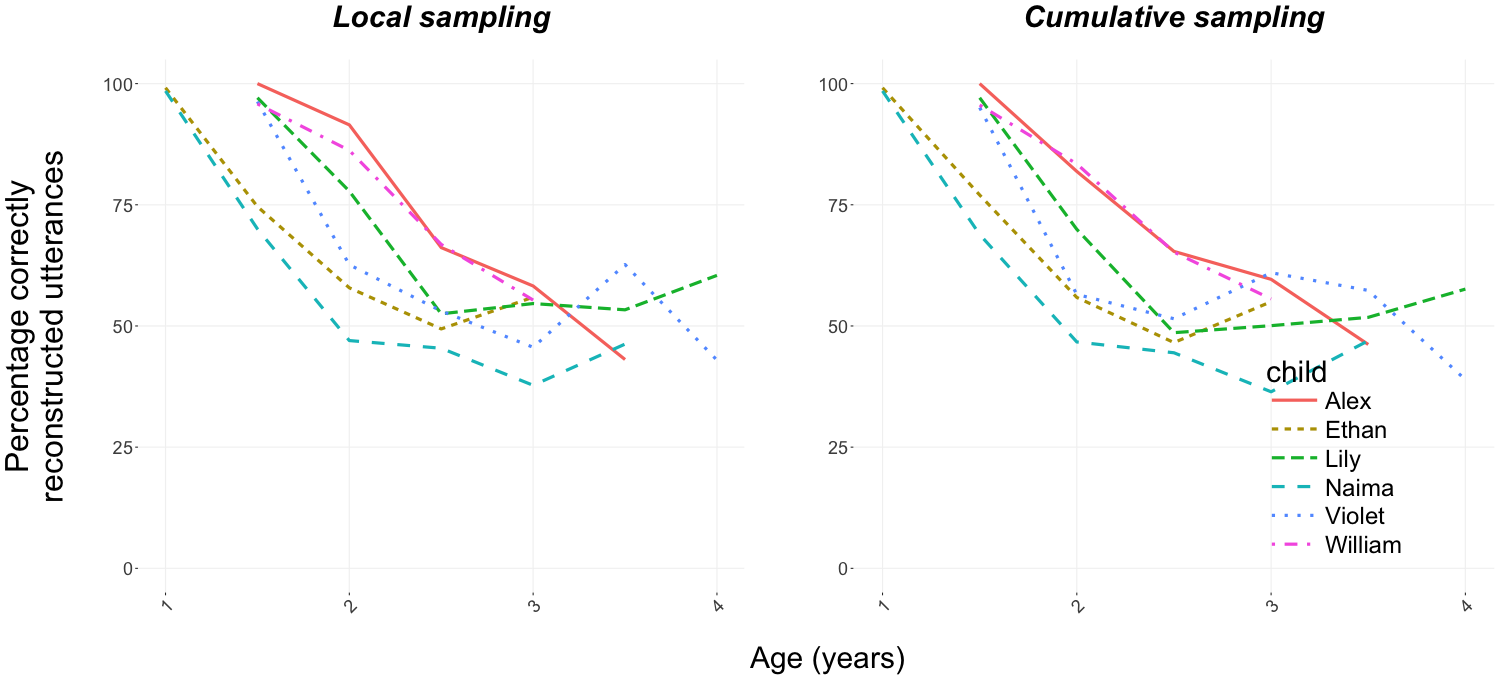
\includegraphics[width=0.95\linewidth]{images/suppl_bothreconperc} 

}

\caption{Uncorrected reconstruction scores across the analyzed age range for local (left) and cumulative (right) sampling while using McCauley and Christiansen's method for handling new words.}\label{fig:smfig1}
\end{figure}

\begin{figure}

{\centering 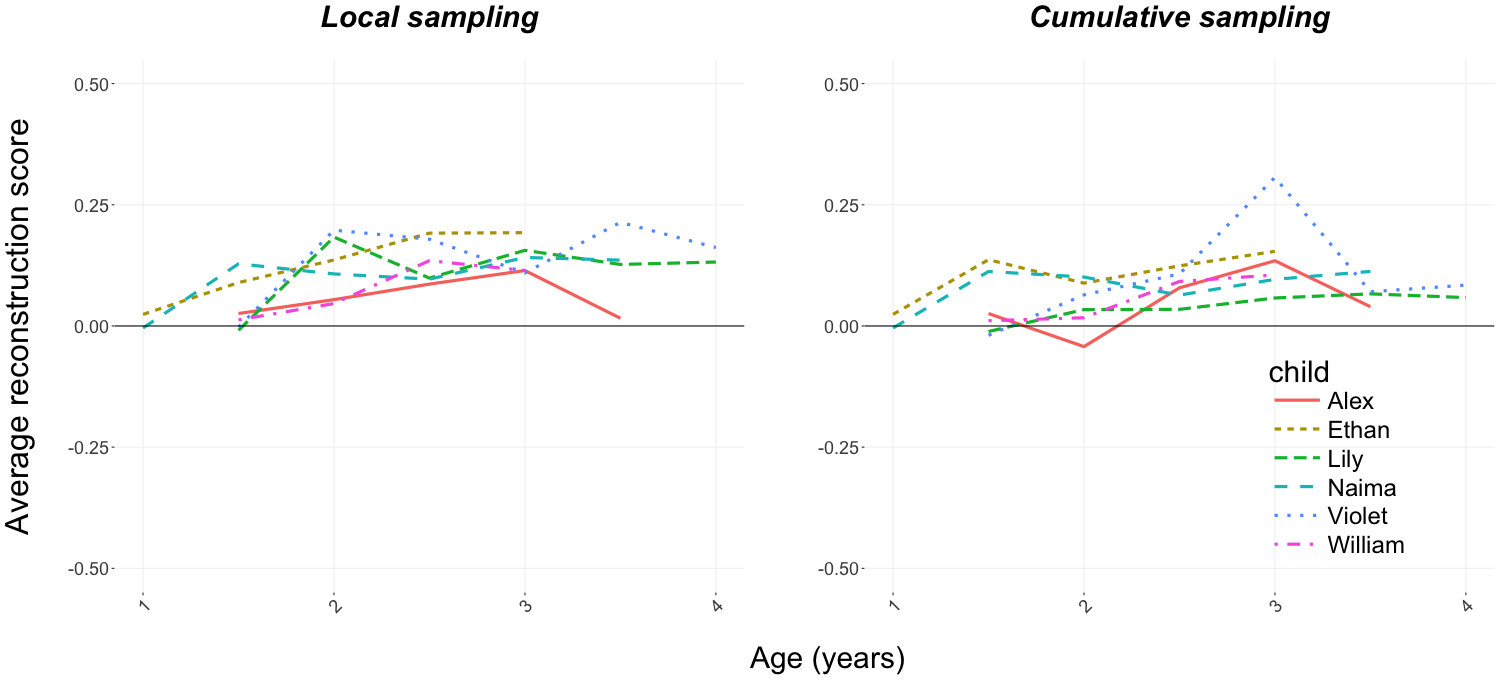
\includegraphics[width=0.95\linewidth]{images/suppl_bothreconscore} 

}

\caption{Corrected reconstruction scores across the analyzed age range for local (left) and cumulative (right) sampling while using McCauley and Christiansen's method for handling new words.}\label{fig:smfig2}
\end{figure}

\newpage

\section{References}\label{references}

\begingroup
\setlength{\parindent}{-0.5in} \setlength{\leftskip}{0.5in}

\hypertarget{refs}{}
\hypertarget{ref-mccauley2011learning}{}
McCauley, S. M., \& Christiansen, M. H. (2011). Learning simple
statistics for language comprehension and production: The CAPPUCCINO
model. \emph{Proceedings of the 33rd Annual Meeting of the Cognitive
Science Society}, 1619--1624.

\hypertarget{ref-mccauley2014acquiring}{}
McCauley, S. M., \& Christiansen, M. H. (2014). Acquiring formulaic
language: A computational model. \emph{The Mental Lexicon}, \emph{9}(3),
419--436.

\endgroup


\end{document}
